% This file was generated with po4a. Translate the source file.
%


\documentclass[a4paper]{article}
\usepackage[T1]{fontenc}
\usepackage[usenames,dvipsnames]{xcolor}
\usepackage{tikz}
\usepackage{framed}
\usepackage{multicol}
\usepackage{fontspec}
\pagestyle{plain}   
\usepackage{ragged2e} 
\usepackage{etoolbox}
\AtBeginEnvironment{multicols}{\RaggedRight}
\definecolor{topblue}{RGB}{29, 56,56}
\definecolor{bottombrown}{RGB}{75, 79, 47}

\usepackage{graphicx}
\usepackage[top=0mm, bottom=0mm, left=0mm, right=0mm]{geometry}
\begin{document}

\hspace{-0.55cm}\begin{tikzpicture}

\setmainfont{DejaVu Serif} \fontsize{1.5cm}{0.9cm} 

\selectfont

\fill [topblue] (0mm,0.5\paperheight) rectangle
(\paperwidth+0.05cm,\paperheight);

\fill [bottombrown] (0mm,0mm) rectangle
(\paperwidth+0.05cm,0.5\paperheight);

\node [below, white] at (0.5\paperwidth, \paperheight-5mm)  {ЗАХИСТИ СВІЙ
EMAIL};

\fontsize{0.65cm}{0.9cm} 

\selectfont

\node [below, white, align=center, text width=0.95\paperwidth] at
(0.5\paperwidth, \paperheight-28mm)  {Масове стеження порушує наші основні
права та призводить до ризику самовисловлення};

\node [below, white, align=center, text width=0.95\paperwidth, font=\bf] at
(0.5\paperwidth, \paperheight-47mm)  {Однак ми не беззахисні і можемо цьому
запобігти};

\node [below, inner sep=0,outer sep=0] at (0.5\paperwidth,
\paperheight-60mm) {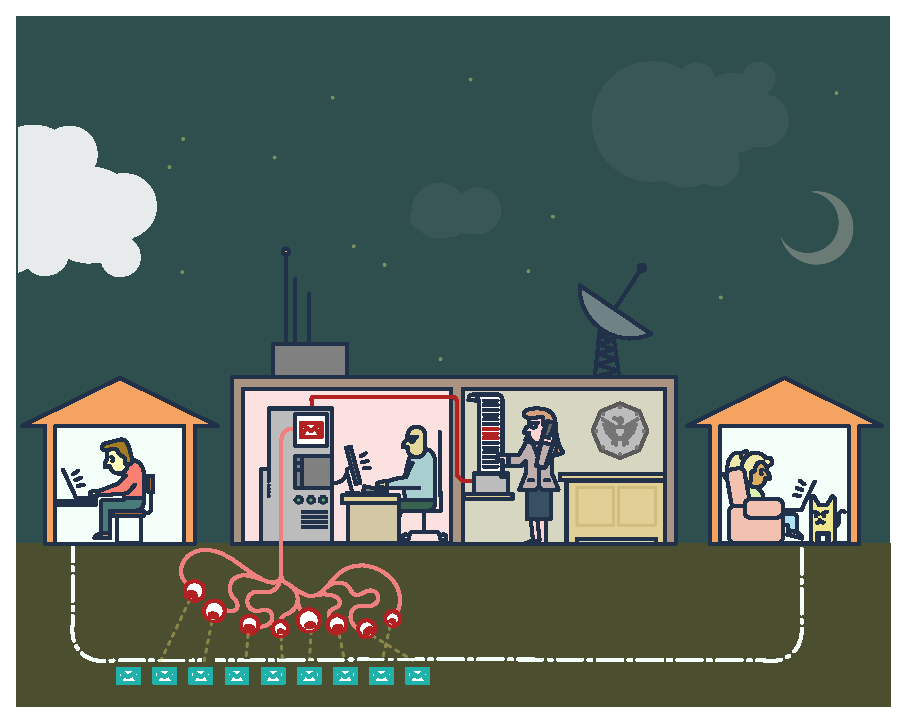
\includegraphics[width=\paperwidth]{leaflet-1_1.eps}};
\fontsize{0.55cm}{0.6cm} \selectfont

\node [below, white, align=center, text width=0.95\paperwidth, font=\bf] at
(0.5\paperwidth, \paperheight-225mm)  { \begin{multicols}{3} Пароль від
вашої пошти - це лише тонкий шар безпеки, який не зможе захистити вас від
передових систем стеження. \par \columnbreak Кожний лист на шляху до
адресата проходить безліч комп'ютерів. Агенства стеження користуються цим,
щоб прочитувати мільйони листів.\par \columnbreak Навіть якщо вам нічого
приховувати, коли ви пересилаєте звичайний лист, ті, з ким ви спілкуєтесь,
також піддаються стеженню.\end{multicols} };

\end{tikzpicture}




\end{document}
